The formulation chapters made their claims about operators. For constant coefficients the standard form's norm grows as $N^{4k}$ against a flat gap; the descriptor's falls to $\Theta(N^2)$ at fixed block weights, at the price of a gap its derivative blocks erode; and a Carleman lift prepares where the doubled space projects. Each claim predicts a filter degree through \Cref{eq:degree}, and the measurements below ask \emph{whether the measured degrees follow those laws, and on which problems}. They use the benchmark problems of \Cref{tab:ladder} with the pipeline and conventions of \Cref{sec:pipeline}, which is validated before any cost is compared. Every result is a classical computation and names its tier, T1, T2 or T3 (\Cref{sec:pipeline-verification}); a gap, a norm or a reference's error is an exact classical computation on the assembled residual. Every problem in both forms is tabulated in \Cref{app:catalogue-results}, and the reproduction of Wu et al.'s panels, which tests the published method rather than our questions, in \Cref{app:reproduction}.

\subsection{Validation of the Pipeline}
\label{sec:results-faithful}

Every number in this chapter is read from one production of $\res{production}{runs}$ runs, $\res{production}{hours}$ hours of computation in all, each of which left a record of its configuration, its outcome and the source code that produced it (\Cref{app:software-campaigns}). Of these, $\res{production}{ok}$ completed; the other $\res{production}{infeasible}$, all circuit simulations, were refused by their own estimates of time and recorded without being attempted. The checks of this section run over those records.

Solved classically through its reference (\Cref{sec:pipeline-reference}), the standard form converges spectrally on every linear benchmark problem: the smallest trusted error of the decoded field is $\res[2,sci]{build/R2a/standard/best}{field_err_linf}$ on R2a at $n=\res{build/R2a/standard/best}{n}$, $\res[2,sci]{build/R4b/standard/best}{field_err_linf}$ on the inhomogeneous R4b at $n=\res{build/R4b/standard/best}{n}$, and $\res[2,sci]{build/R5b/standard/best}{field_err_linf}$ on the heat equation at $n=\res{build/R5b/standard/best}{n}$ per axis. The descriptor, whose kernel is the standard form's (\Cref{thm:kernel-equivalence}), reaches $\res[2,sci]{build/R2a/descriptor/best}{field_err_linf}$ on R2a. Beyond its best resolution the standard form's error rises again, to $\res[2,sci]{build/R2a/standard/n10}{field_err_linf}$ on R2a at $n=10$, where the descriptor's is $\res[2,sci]{build/R2a/descriptor/n10}{field_err_linf}$. The rise is consistent with rounding error amplified by the conditioning of a residual whose norm grows as $N^4$, an early sign of the Hamiltonian's cost of \Cref{sec:results-scaling}.

\paragraph{The circuits encode the operators.} All $\res{verification/all}{count}$ verifications, $\res{verification/exact}{count}$ exact, $\res{verification/probe}{count}$ by probe and $\res{verification/ir}{count}$ by \gls{ir}, meet their mode's tolerance (\Cref{tab:verification-modes}) by at least four orders of magnitude, the least margin a factor of $\res[2,sci]{verification/all}{least_margin}$ (\Cref{fig:verification-accuracy}). The exact mode's worst entrywise error is $\res[2,sci]{encode/R6a/standard/n3}{verify_max_error}$, and its widest verification, a whole reflection of the reproduction on $\res{encode/R4d/faithful/standard/n3}{n_qubits_total}$ qubits, is accurate to $\res[2,sci]{encode/R4d/faithful/standard/n3}{verify_max_error}$. The probe mode's worst is $\res[2,sci]{encode/R10c-M12/descriptor/n2/carleman=2/verify=probe}{verify_max_error}$, on a Navier--Stokes lift's reflection of $\res{encode/R10c-M12/descriptor/n2/carleman=2/verify=probe}{n_qubits_total}$ qubits, and the \gls{ir} mode verifies the tensor layout's coupling on $\res{lift/R10c-M316/standard/n0/carleman=2/lift=tensor/verify=ir}{modes}$ modes to $\res[2,sci]{lift/R10c-M316/standard/n0/carleman=2/lift=tensor/verify=ir}{verify_max_error}$. Every composed Hamiltonian of at most 24 qubits is therefore verified whole, and every lift and coupling by its terms at any size. The $\res{verification/none}{count}$ wider reflections, those of the two-axis descriptor problems from $\res{encode/R5b/descriptor/n2x2/verify=none}{n_qubits_total}$ qubits and of the larger lifts, are built and counted but not independently verified (\Cref{sec:pipeline-verification}).

\paragraph{The circuit computes the emulation.} On all $\res{agreement/T1/minimax}{count}$ circuit simulations with the minimax filter the simulated output agrees with the exact emulation's before normalising, within the bar of $10^{-10}$. The worst difference is $\res[2,sci]{stateprep/R4a/descriptor/n3/T1/filter=minimax}{filtered_agreement}$ in the descriptor (R4a at $n=3$, degree $\res{stateprep/R4a/descriptor/n3/T1/filter=minimax}{degree}$), $\res[2,sci]{stateprep/R4a/standard/n2/T1/filter=minimax}{filtered_agreement}$ in the standard form (R4a at $n=2$, degree $\res{stateprep/R4a/standard/n2/T1/filter=minimax}{degree}$) and $\res[2,sci]{stateprep/R9c-M4/descriptor/n2/T1/carleman=2/filter=minimax}{filtered_agreement}$ on a Carleman lift (Burgers on four modes, $\res{stateprep/R9c-M4/descriptor/n2/T1/carleman=2/filter=minimax}{n_qubits}$ qubits). Where both run, this confirms the argument of \Cref{sec:pipeline-verification} that the exact emulation is the circuit's output, which licenses the emulation beyond the widths simulated. The widest circuit simulated for a problem as run has $\res{stateprep/R4d/descriptor/n3/T1/filter=minimax}{n_qubits}$ qubits. The two-axis descriptor circuits, of $\res{stateprep/R5b/descriptor/n2x2/T1/filter=minimax}{n_qubits}$ to $\res{stateprep/R5a/descriptor/n2x2/T1/filter=minimax}{n_qubits}$ qubits, are beyond the simulation budget, the narrowest estimated at $\res[2]{stateprep/R5b/descriptor/n2x2/T1/filter=minimax}{predicted_seconds}$\,s against a budget of $\res[2]{stateprep/R5b/descriptor/n2x2/T1/filter=minimax}{budget_seconds}$\,s: a limit of the classical simulation, not of the circuit. Of the reproduction's $\res{agreement/T1/qite}{count}$ imaginary-time simulations, $\res{agreement/T1/qite}{misses}$, at degrees of order $10^5$, miss the bar (\Cref{app:repro-t1}).

\paragraph{Every prepared state meets its target.} Each of the $\res{preparation/T2/minimax}{trusted}$ trusted preparations by exact emulation meets $\varepsilon$ and its a priori bound, in both forms, on every linear problem and every Carleman lift, and its decoded field meets the error budget of \Cref{eq:error-budget} (\Cref{tab:catalogue-results}). The bound is tight: on R2a in the descriptor at $n=8$ the infidelity is $\res[2,sci]{stateprep/R2a/descriptor/n8/T2/filter=minimax}{infidelity}$ against the bound $(1-\gamma^2)\varepsilon^2/\gamma^2=\res[2,sci]{stateprep/R2a/descriptor/n8/T2/filter=minimax}{infidelity_bound}$ of \Cref{sec:pipeline-filter}. The field's error falls spectrally with $n$ until it meets the error the filter leaves, which is the same at every $n$, and then holds, as the plot of the error, $\varepsilon_{\mathrm{disc}}$ and the budget's terms against $n$ in \Cref{fig:decoded-field} shows: on R2a in the descriptor it is $\res[2,sci]{stateprep/R2a/descriptor/n4/T2/filter=minimax}{field_err_linf}$ at $n=4$ and $\res[2,sci]{stateprep/R2a/descriptor/n8/T2/filter=minimax}{field_err_linf}$ at $n=8$, while the discretisation's own error falls to $\res[2,sci]{stateprep/R2a/descriptor/n8/T2/filter=minimax}{eps_disc}$. From $n=4$ the prepared field's accuracy is set by $\varepsilon$, which the degree pays for logarithmically (\Cref{eq:minimax-degree}), and a larger $n$ gains nothing. The budget, $\res[2,sci]{stateprep/R2a/descriptor/n8/T2/filter=minimax}{field_budget}$ there, is conservative by more than an order of magnitude, consistent with a readout bound that takes the state's worst direction rather than its actual one, and the margin widens with $n$: the bound's amplification grows from $\res[3]{stateprep/R2a/descriptor/n4/T2/filter=minimax}{kappa_read}$ at $n=4$ to $\res[3]{stateprep/R2a/descriptor/n8/T2/filter=minimax}{kappa_read}$ at $n=8$ while the prepared field's error does not.

\paragraph{What answer independence costs.} The geometric initial state of \Cref{eq:geometric-state} assumes that the solution's coefficients decay geometrically, and overlaps well where they do: on R1 at $n=3$, $\gamma^2=\res[3]{stateprep/R1/standard/n3/T2/filter=minimax}{gamma2}$, against $\res[2,sci]{stateprep/R1/standard/n3/T2/kind=uniform/filter=minimax/initial-state-control}{gamma2}$ for the uniform state and $\res[2]{stateprep/R1/standard/n3/T2/kind=random/filter=minimax/initial-state-control}{gamma2}$ for a random one. On Legendre's equation R3a, whose solution is the polynomial $P_4$, the uniform state does better, $\res[3]{stateprep/R3a/standard/n3/T2/kind=uniform/filter=minimax/initial-state-control}{gamma2}$ against the geometric state's $\res[3]{stateprep/R3a/standard/n3/T2/filter=minimax}{gamma2}$ (exact emulation, T2). The degree does not depend on the initial state, so every control meets $\varepsilon$ at the same degree and a poor guess costs the amplification factor $1/\gamma$ of \Cref{eq:total-cost}. An underestimated spectral edge raises the degree as the inverse square root of the gap and keeps the target; the study on R2a, in which Wu et al.'s time rule falls short of $\varepsilon$, is given in \Cref{app:edge-study}.

\paragraph{The filter.} On synthetic spectra with the ground state at the edge, imaginary time needs $\res[3]{filters/synthetic/edge}{low}$--$\res[3]{filters/synthetic/edge}{high}$ times the minimax filter's degree at equal suppression, whatever the gap, and on the benchmark problems compared the certified ratio lies in that range in both forms (exact emulation, T2). At equal measured infidelity the margin is smaller, and at $\varepsilon=10^{-4}$ imaginary time needs fewer degrees on three of the eight cases (\Cref{app:filter-study}). The choice of filter therefore sets the degree's constant and leaves its growth with $N$ unchanged.

The pipeline is therefore faithful wherever it can be checked, and the differences measured in the rest of this chapter are differences between residuals.

\subsection{The Cost of the Two Forms}
\label{sec:results-scaling}

\Cref{tab:headline} separates the two costs of \Cref{sec:standard} on R2a ($f''+4f'+4f=0$) at $n=8$, the largest resolution estimated for every encoding. The first two columns encode one Hamiltonian, $\Hstd$, so they share its norm, its gap and its ideal-bound degree, and differ only in how tightly they encode it: Wu et al.'s encoding exceeds the residual's norm by a factor of $\res[2,sci]{looseness/stateprep/R2a/standard/n8/T3/filter=minimax/encoder=published}{alpha_ratio}$ and the structured encoding by $\res[3]{looseness/stateprep/R2a/standard/n8/T3/filter=minimax}{alpha_ratio}$, and the degree falls between them by the same factor. That factor is the encoder's cost. The descriptor's column is a different Hamiltonian with the same kernel, encoded within a few per cent of its norm. The distance between the standard form's ideal-bound degree and the descriptor's is the Hamiltonian's cost, which no encoding of $\Hstd$ recovers (\Cref{prop:ideal-degree}).

\begin{table}[htbp]
    \centering
    \caption[The encoder's cost against the Hamiltonian's cost on R2a at $n=8$]{\textbf{The encoder's cost and the Hamiltonian's cost are separate, and only the second is the reformulation's to remove.} R2a ($f''+4f'+4f=0$) at $n=8$, minimax filter at $\varepsilon=10^{-6}$. The first two columns encode the same $\Hstd$, so their norm, gap and ideal-bound degree coincide; the third is the descriptor's $\Hdesc$, with the same kernel. $\|H\|$, spectral norm; $\Delta$, spectral gap; $\alpha_R/\|R\|_2$, looseness, the encoding's subnormalisation over the residual's norm; ancilla, those of the reflection $V$; query, one walk step; growth, the exponent of $N=2^n$ between $n=7$ and $8$; $\alpha_R=\|R\|_2$, the ideal-encoding bound. Norms, gaps and looseness: exact classical computation. Degrees, qubits and gate counts: resource estimates (T3), the descriptor's degree confirmed by exact emulation (T2).}
    \label{tab:headline}
    \small
    \setlength{\tabcolsep}{5pt}
    \begin{tabular}{@{}l l l l@{}}
        \toprule
        & \multicolumn{2}{c}{Standard form, $\Hstd$} & Descriptor, $\Hdesc$ \\
        \cmidrule(lr){2-3}\cmidrule(lr){4-4}
        & Wu et al.'s encoding & structured encoding & \\
        \midrule
        $\|H\|$, its law & $\Theta(N^8)$ & $\Theta(N^8)$ & $\Theta(N^2)$ \\
        $\|H\|$ & $\res[2,sci]{build/R2a/standard/n8}{hamiltonian_norm}$ & $\res[2,sci]{build/R2a/standard/n8}{hamiltonian_norm}$ & $\res[2,sci]{build/R2a/descriptor/n8}{hamiltonian_norm}$ \\
        Gap $\Delta$ & $\res[3]{build/R2a/standard/n8}{gap}$ & $\res[3]{build/R2a/standard/n8}{gap}$ & $\res[3]{build/R2a/descriptor/n8}{gap}$ \\
        Looseness $\alpha_R/\|R\|_2$ & $\res[2,sci]{looseness/stateprep/R2a/standard/n8/T3/filter=minimax/encoder=published}{alpha_ratio}$ & $\res[3]{looseness/stateprep/R2a/standard/n8/T3/filter=minimax}{alpha_ratio}$ & $\res[3]{looseness/stateprep/R2a/descriptor/n8/T3/filter=minimax}{alpha_ratio}$ \\
        Encoding & approximate, $\mathcal{O}(N^{-5})$ & exact & exact (no $\G$) \\
        Qubits & $\res{stateprep/R2a/standard/n8/T3/filter=minimax/encoder=published}{n_qubits}$ & $\res{stateprep/R2a/standard/n8/T3/filter=minimax}{n_qubits}$ & $\res{stateprep/R2a/descriptor/n8/T3/filter=minimax}{n_qubits}$ \\
        Ancilla & $\res{query/stateprep/R2a/standard/n8/T3/filter=minimax/encoder=published}{ancilla}$ & $\res{query/stateprep/R2a/standard/n8/T3/filter=minimax}{ancilla}$ & $\res{query/stateprep/R2a/descriptor/n8/T3/filter=minimax}{ancilla}$ \\
        Two-qubit gates per query & $\res{query/stateprep/R2a/standard/n8/T3/filter=minimax/encoder=published}{gates}$ & $\res{query/stateprep/R2a/standard/n8/T3/filter=minimax}{gates}$ & $\res{query/stateprep/R2a/descriptor/n8/T3/filter=minimax}{gates}$ \\
        Degree, as built & $\res[2,sci]{stateprep/R2a/standard/n8/T3/filter=minimax/encoder=published}{degree}$ & $\res[2,sci]{stateprep/R2a/standard/n8/T3/filter=minimax}{degree}$ & $\res{stateprep/R2a/descriptor/n8/T3/filter=minimax}{degree}$ \\
        Degree, $\alpha_R=\|R\|_2$ & $\res[2,sci]{stateprep/R2a/standard/n8/T3/filter=minimax/encoder=published}{ideal_degree}$ & $\res[2,sci]{stateprep/R2a/standard/n8/T3/filter=minimax}{ideal_degree}$ & $\res{stateprep/R2a/descriptor/n8/T3/filter=minimax}{ideal_degree}$ \\
        Degree's growth, as built & $N^{\res[3]{stateprep/R2a/standard/growth/T3/filter=minimax/encoder=published}{degree}}$ & $N^{\res[3]{stateprep/R2a/standard/growth/T3/filter=minimax}{degree}}$ & $N^{\res[3]{stateprep/R2a/descriptor/growth/T3/filter=minimax}{degree}}$ \\
        Degree's growth, $\alpha_R=\|R\|_2$ & $N^{\res[3]{stateprep/R2a/standard/growth/T3/filter=minimax/encoder=published}{ideal_degree}}$ & $N^{\res[3]{stateprep/R2a/standard/growth/T3/filter=minimax}{ideal_degree}}$ & $N^{\res[3]{stateprep/R2a/descriptor/growth/T3/filter=minimax}{ideal_degree}}$ \\
        Two-qubit gates, preparation & $\res[2,sci]{stateprep/R2a/standard/n8/T3/filter=minimax/encoder=published}{gate_count}$ & $\res[2,sci]{stateprep/R2a/standard/n8/T3/filter=minimax}{gate_count}$ & $\res[2,sci]{stateprep/R2a/descriptor/n8/T3/filter=minimax}{gate_count}$ \\
        \bottomrule
    \end{tabular}
\end{table}

\Cref{fig:scaling-headline} follows the three encodings in $N$. Between $n=7$ and $8$, $\|\Hstd\|$ rises from $\res[2,sci]{build/R2a/standard/n7}{hamiltonian_norm}$ by a factor $2^8$ and $\|\Hdesc\|$ from $\res[2,sci]{build/R2a/descriptor/n7}{hamiltonian_norm}$ by $2^2$, while both gaps hold (\Cref{sec:standard-hamiltonian,sec:descriptor-spectrum}); the degree's exponents in \Cref{tab:headline}, two-point slopes of a degree with logarithmic factors, are consistent with $\tilde\Theta(N^{10})$, $\tilde\Theta(N^4)$ and $\tilde\Theta(N)$. The separation between Wu et al.'s curve and the structured one grows as $N^{3k}=N^6$, and an exact encoding of the same Hamiltonian removes it; that between the structured curve and the descriptor's grows as $N^3$, and only a different Hamiltonian removes it.

\begin{figure}[htbp]
    \centering
    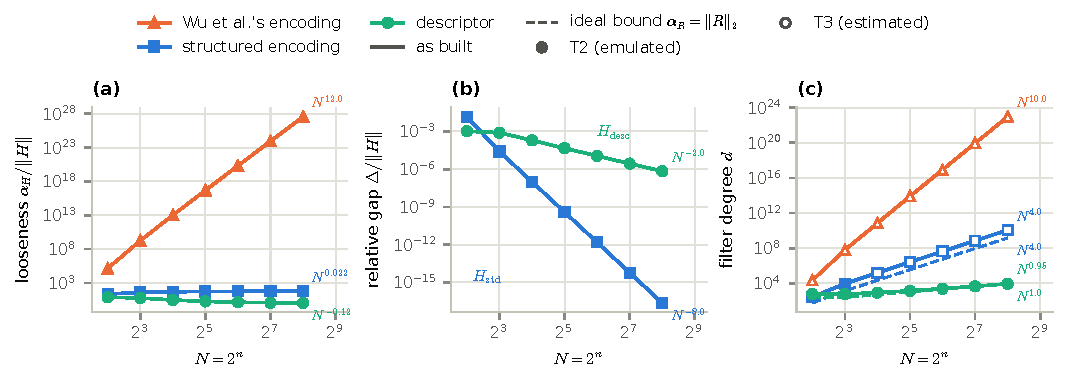
\includegraphics[width=\linewidth]{Figs/scaling_headline.pdf}
    \caption[Looseness, relative gap and degree against $N$ on R2a]{\textbf{The encoder's cost and the Hamiltonian's cost are two separate gaps on one plot.} R2a against $N=2^n$, $n=2$--$8$, log--log, for Wu et al.'s encoding, the structured encoding and the descriptor. (a) The encoding's looseness $\alpha_H/\|H\|=(\alpha_R/\|R\|_2)^2$: growing as $N^{12}$ for Wu et al.'s encoding, bounded for the structured, falling towards one for the descriptor. (b) The relative gap $\Delta/\|H\|$: $\Theta(N^{-8})$ for $\Hstd$, $\Theta(N^{-2})$ for $\Hdesc$. (c) The filter's degree as built (solid) and at the ideal-encoding bound $\alpha_R=\|R\|_2$ (dashed); it is about $\tfrac12\sqrt{\alpha_H/\Delta}\,\ln(2/\varepsilon)$, so (c) is the square root of (a) over (b). The vertical distance between Wu et al.'s and the structured curves is the encoder's cost; that between the structured and the descriptor curves at the ideal bound is the Hamiltonian's cost. Exact emulation (T2, filled) on the resolutions emulated, the descriptor to $n=8$ and the standard form to $n=3$, the grid of its imaginary-time reproduction; resource estimates (T3, open) beyond. Norms and gaps are exact classical computations.}
    \label{fig:scaling-headline}
\end{figure}

\Cref{tab:growth} extends the measurement to the classes of \Cref{tab:descriptor-regimes}, with every linear problem and the coupled oscillator R7 in \Cref{tab:catalogue-growth}. In the standard form on one axis, with constant coefficients, the degree grows as $N^{2k}$ as built and at the ideal bound alike: the structured encoding holds the encoder's cost to a constant, and what remains is the Hamiltonian's. In the descriptor, on every regular problem (\Cref{def:regular}), it grows as about $N$, its exponents between $\res[3]{stateprep/R4d/descriptor/growth/T3/filter=minimax}{degree}$ (R4d) and $\res[3]{stateprep/R1/descriptor/growth/T3/filter=minimax}{degree}$ (R1) as built and within a few per cent of one at the ideal bound. The stiff R2c is the exception as built, at $N^{\res[3]{stateprep/R2c/descriptor/growth/T3/filter=minimax}{degree}}$, because its degree is still rising towards the asymptotic regime at $n=8$; its ideal-bound exponent is already $\res[3]{stateprep/R2c/descriptor/growth/T3/filter=minimax}{ideal_degree}$. On the singular problems (R3, R4a) the descriptor's degree grows as about $N^2$, the price of the rescaling's $\zeta\propto N$ (\Cref{sec:descriptor-rescaling}). On two axes it grows faster than $N^2$ per axis yet more slowly than the standard form's, between the least settled resolutions in the table, $n=4$ and $5$ per axis.

\begin{table}[htbp]
    \centering
    \caption[Growth of the filter's degree with $N$, by class of problem]{\textbf{The descriptor's degree grows as about $N$ where the equation controls every carried derivative; the standard form's grows as $N^{2k}$ on one axis with constant coefficients.} Exponent of $N=2^n$ in the minimax filter's degree between the two largest resolutions estimated ($n=7\to8$ on one axis, $n=4\to5$ per axis on two), as built and at the ideal-encoding bound $\alpha_R=\|R\|_2$, for representatives of each class of \Cref{tab:descriptor-regimes} (every problem: \Cref{tab:catalogue-growth}). $k$, equation order; regular, singular: the leading coefficient without and with a zero on $[-1,1]$ (\Cref{def:regular}). The standard form's as-built exponent on R3a is its lifted multiplier's looseness; at the ideal bound both forms grow as $N^2$ there. Two-point slopes of a degree with logarithmic factors: consistent with the laws, not fits of them. Resource estimates (T3).}
    \label{tab:growth}
    \small
    \begin{tabular}{@{}l l r r r r@{}}
        \toprule
        & & \multicolumn{2}{c}{Standard} & \multicolumn{2}{c}{Descriptor} \\
        \cmidrule(lr){3-4}\cmidrule(lr){5-6}
        Class & Problem & As built & Ideal & As built & Ideal \\
        \midrule
        First order, $k=1$ & R1 & $\res[3]{stateprep/R1/standard/growth/T3/filter=minimax}{degree}$ & $\res[3]{stateprep/R1/standard/growth/T3/filter=minimax}{ideal_degree}$ & $\res[3]{stateprep/R1/descriptor/growth/T3/filter=minimax}{degree}$ & $\res[3]{stateprep/R1/descriptor/growth/T3/filter=minimax}{ideal_degree}$ \\
        \addlinespace
        Second order, regular & R2a & $\res[3]{stateprep/R2a/standard/growth/T3/filter=minimax}{degree}$ & $\res[3]{stateprep/R2a/standard/growth/T3/filter=minimax}{ideal_degree}$ & $\res[3]{stateprep/R2a/descriptor/growth/T3/filter=minimax}{degree}$ & $\res[3]{stateprep/R2a/descriptor/growth/T3/filter=minimax}{ideal_degree}$ \\
         & R2c & $\res[3]{stateprep/R2c/standard/growth/T3/filter=minimax}{degree}$ & $\res[3]{stateprep/R2c/standard/growth/T3/filter=minimax}{ideal_degree}$ & $\res[3]{stateprep/R2c/descriptor/growth/T3/filter=minimax}{degree}$ & $\res[3]{stateprep/R2c/descriptor/growth/T3/filter=minimax}{ideal_degree}$ \\
        \addlinespace
        Second order, singular & R3a & $\res[3]{stateprep/R3a/standard/growth/T3/filter=minimax}{degree}$ & $\res[3]{stateprep/R3a/standard/growth/T3/filter=minimax}{ideal_degree}$ & $\res[3]{stateprep/R3a/descriptor/growth/T3/filter=minimax}{degree}$ & $\res[3]{stateprep/R3a/descriptor/growth/T3/filter=minimax}{ideal_degree}$ \\
         & R4a & $\res[3]{stateprep/R4a/standard/growth/T3/filter=minimax}{degree}$ & $\res[3]{stateprep/R4a/standard/growth/T3/filter=minimax}{ideal_degree}$ & $\res[3]{stateprep/R4a/descriptor/growth/T3/filter=minimax}{degree}$ & $\res[3]{stateprep/R4a/descriptor/growth/T3/filter=minimax}{ideal_degree}$ \\
        \addlinespace
        Two axes, per axis & R5a & $\res[3]{stateprep/R5a/standard/growth/T3/filter=minimax}{degree}$ & $\res[3]{stateprep/R5a/standard/growth/T3/filter=minimax}{ideal_degree}$ & $\res[3]{stateprep/R5a/descriptor/growth/T3/filter=minimax}{degree}$ & $\res[3]{stateprep/R5a/descriptor/growth/T3/filter=minimax}{ideal_degree}$ \\
         & R5b & $\res[3]{stateprep/R5b/standard/growth/T3/filter=minimax}{degree}$ & $\res[3]{stateprep/R5b/standard/growth/T3/filter=minimax}{ideal_degree}$ & $\res[3]{stateprep/R5b/descriptor/growth/T3/filter=minimax}{degree}$ & $\res[3]{stateprep/R5b/descriptor/growth/T3/filter=minimax}{ideal_degree}$ \\
        \bottomrule
    \end{tabular}
\end{table}

\paragraph{The reversals.} Two comparisons reverse at the ideal bound, and both are findings (\Cref{fig:gap-cases}). On the four Legendre problems R3 the standard form needs the smaller degree (\Cref{tab:catalogue-t3}): on R3a at $n=8$, $\res[2,sci]{stateprep/R3a/standard/n8/T3/filter=minimax}{ideal_degree}$ against the descriptor's $\res[2,sci]{stateprep/R3a/descriptor/n8/T3/filter=minimax}{ideal_degree}$. As built the order is the other way, $\res[2,sci]{stateprep/R3a/standard/n8/T3/filter=minimax}{degree}$ against $\res[2,sci]{stateprep/R3a/descriptor/n8/T3/filter=minimax}{degree}$, because the structured encoding pays for R3's lifted multiplier in full, so on R3 the descriptor's as-built advantage is the encoder's. Both forms prepare R3a's exact kernel $P_4$ from $n=3$, and both ideal-bound degrees grow as $N^2$, while the standard form's as-built degree grows as $N^4$ (\Cref{tab:growth}). The reversal is R3's and not that of every vanishing coefficient: R3a's $\|\Hstd\|$ grows only as $N^4$, from $\res[2,sci]{build/R3a/standard/n7}{hamiltonian_norm}$ at $n=7$ to $\res[2,sci]{build/R3a/standard/n8}{hamiltonian_norm}$ at $n=8$, while that of R4a, whose coefficient $x-1$ vanishes at one end only, grows as $N^8$, from $\res[2,sci]{build/R4a/standard/n7}{hamiltonian_norm}$ to $\res[2,sci]{build/R4a/standard/n8}{hamiltonian_norm}$, and there the descriptor's ideal-bound degree is the lower, $\res[2,sci]{stateprep/R4a/descriptor/n8/T3/filter=minimax}{ideal_degree}$ against $\res[2,sci]{stateprep/R4a/standard/n8/T3/filter=minimax}{ideal_degree}$. The second reversal is the heat equation R5b, whose reference is trusted from $n=4$ per axis. There the descriptor's degree is the higher, $\res{stateprep/R5b/descriptor/n4x4/T3/filter=minimax}{degree}$ against $\res{stateprep/R5b/standard/n4x4/T3/filter=minimax}{degree}$ as built and $\res{stateprep/R5b/descriptor/n4x4/T3/filter=minimax}{ideal_degree}$ against $\res{stateprep/R5b/standard/n4x4/T3/filter=minimax}{ideal_degree}$ at the ideal bound; at $n=5$ it is the lower as built, $\res[2,sci]{stateprep/R5b/descriptor/n5x5/T3/filter=minimax}{degree}$ against $\res[2,sci]{stateprep/R5b/standard/n5x5/T3/filter=minimax}{degree}$, and level at the ideal bound, $\res[2,sci]{stateprep/R5b/descriptor/n5x5/T3/filter=minimax}{ideal_degree}$ against $\res[2,sci]{stateprep/R5b/standard/n5x5/T3/filter=minimax}{ideal_degree}$. Its exponent per axis is the smaller (\Cref{tab:growth}), so the order should settle in the descriptor's favour at larger $n$, an extrapolation. Two axes do not by themselves reverse the comparison: on the Laplace equation R5a the descriptor's ideal-bound degree is the lower at $n=4$ and $5$ per axis, $\res[2,sci]{stateprep/R5a/descriptor/n5x5/T3/filter=minimax}{ideal_degree}$ against $\res[2,sci]{stateprep/R5a/standard/n5x5/T3/filter=minimax}{ideal_degree}$ at $n=5$.

\begin{figure}[htbp]
    \centering
    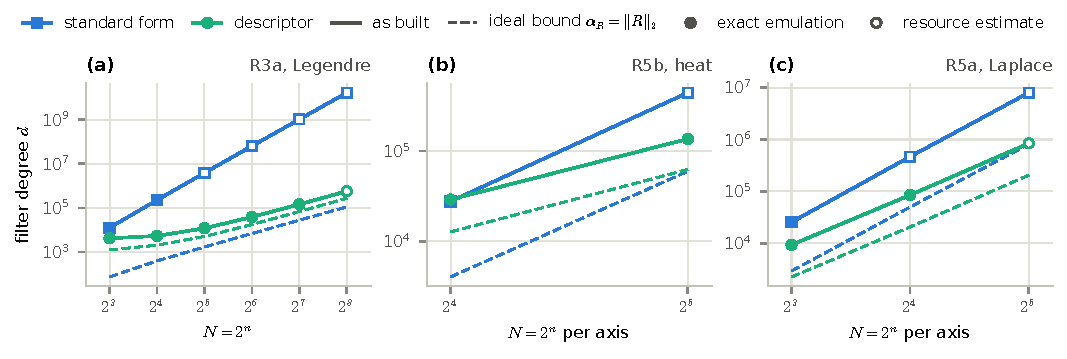
\includegraphics[width=\linewidth]{Figs/gap_cases.pdf}
    \caption[The ideal-bound reversals]{\textbf{At the ideal-encoding bound the standard form's degree is the lower on R3a at every $n$ and on the heat equation R5b at $n=4$ per axis; on the Laplace equation R5a it is not.} The minimax filter's degree against $N$ (per axis on R5), standard (squares) and descriptor (circles), as built (solid) and at the ideal-encoding bound $\alpha_R=\|R\|_2$ (dashed), at the resolutions whose reference is trusted. (a) R3a, Legendre's equation: the descriptor lower as built, higher at the ideal bound. At the ideal bound both degrees grow as $N^2$; as built the standard form's grows as $N^4$, its encoding paying for R3a's lifted multiplier in full. (b) R5b, heat: higher at $n=4$ per axis in both comparisons; at $n=5$ lower as built and level at the ideal bound. (c) R5a, Laplace: lower in both comparisons. Exact emulation (T2, filled) where emulated, resource estimates (T3, open) beyond.}
    \label{fig:gap-cases}
\end{figure}

\paragraph{Queries and gates.} The degree counts queries, and a query's gates differ between the forms. On R2a one query of the descriptor costs more two-qubit gates than one of the structured standard form at every resolution built and verified, $\res{encode/R2a/descriptor/n2}{cx_count}$ against $\res{encode/R2a/standard/n2}{cx_count}$ at $n=2$ and $\res{encode/R2a/descriptor/n5/verify=probe}{cx_count}$ against $\res{encode/R2a/standard/n5/verify=probe}{cx_count}$ at $n=5$, having more terms and a block register; its count grows more slowly, and the estimates at $n=8$ put the two level (\Cref{tab:headline}). On R3a, whose lifted multiplier the structured encoding pays for in full, the descriptor's query is the cheaper from $n=4$: $\res{encode/R3a/descriptor/n4/verify=probe}{cx_count}$ against $\res{encode/R3a/standard/n4/verify=probe}{cx_count}$ at $n=4$ and $\res{encode/R3a/descriptor/n5/verify=probe}{cx_count}$ against $\res{encode/R3a/standard/n5/verify=probe}{cx_count}$ at $n=5$. The ancilla's growth, $\mathcal{O}(\log n)$ against $n$ (\Cref{sec:descriptor-cost}), first shows at $n=8$ (\Cref{tab:headline}); at $n=2$ and $5$ the descriptor's reflection on R2a needs $\res{encode/R2a/descriptor/n2}{n_anc_qubits}$ and $\res{encode/R2a/descriptor/n5/verify=probe}{n_anc_qubits}$ ancilla against the standard form's $\res{encode/R2a/standard/n2}{n_anc_qubits}$ and $\res{encode/R2a/standard/n5/verify=probe}{n_anc_qubits}$. On constant-coefficient problems the descriptor's advantage therefore lies in the number of queries, which dominates the preparation's gate count (\Cref{tab:headline}). The standard form's degrees at $n=8$ are resource estimates far beyond the $2^{20}$ that exact emulation reaches (\Cref{sec:pipeline-verification}), a limit of the classical emulation that does not bound the circuit; the descriptor's agree with exact emulation through $n=8$.

The standard form's cost is therefore measured as well as argued: with Wu et al.'s encoding it is mostly the encoder's, an exact encoding removes that part, and what remains, $\tilde\Theta(N^{2k})$ in the degree for constant coefficients on one axis, is the Hamiltonian's. The descriptor removes the Hamiltonian's part on regular problems; on singular ones its degree still grows as $N^2$, and on R3 at the ideal bound the standard form's is the lower.

\subsection{The Descriptor's Gap and Its Rescaling}
\label{sec:results-gap}

\Cref{sec:descriptor-gap} traced the descriptor's gap to the derivatives it carries: the gap shrinks where the solution's derivatives are large and closes on singular problems and on two axes, and block rescaling restores it on one axis only. \Cref{fig:gap-rescaling} measures this on every panel. Unscaled, the gap on the physical subspace at $n=8$ is $\res[3]{build/R2a/descriptor/n8/unscaled}{gap}$ on R2a but $\res[2,sci]{build/R2c/descriptor/n8/unscaled}{gap}$ on the stiff R2c and $\res[2,sci]{build/R3a/descriptor/n8/unscaled}{gap}$ on the singular R3a, and the field block holds as little as $\res[2,sci]{build/R2c/descriptor/n8/unscaled}{field_weight}$ of the ground state on R2c. Rescaled, the gaps are $\res[3]{build/R2a/descriptor/n8}{gap}$, $\res[3]{build/R2c/descriptor/n8}{gap}$ and $\res[3]{build/R3a/descriptor/n8}{gap}$ and the field block's weights $\res[3]{build/R2a/descriptor/n8}{field_weight}$, $\res[3]{build/R2c/descriptor/n8}{field_weight}$ and $\res[3]{build/R3a/descriptor/n8}{field_weight}$. Every reference here is trusted in both versions, so the rescaling changes the filter's work and not the prepared field. On two axes the Laplace equation's rescaled gap falls from $\res[3]{build/R5a/descriptor/n3x3}{gap}$ at $n=3$ per axis, where its reference is first trusted, to $\res[2,sci]{build/R5a/descriptor/n5x5}{gap}$ at $n=5$, against $\res[2,sci]{build/R5a/descriptor/n3x3/unscaled}{gap}$ and $\res[2,sci]{build/R5a/descriptor/n5x5/unscaled}{gap}$ unscaled; at $n=5$ per axis the heat and wave equations' rescaled gaps are $\res[2,sci]{build/R5b/descriptor/n5x5}{gap}$ and $\res[2,sci]{build/R5c/descriptor/n5x5}{gap}$. That is a negative finding: on two axes block rescaling slows the gap's fall and does not stop it. Rescaling also raises the ceiling $\gamma\le w_f^{1/2}$ on the initial state's overlap (\Cref{sec:pipeline-filter}), though how near the geometric state comes to it depends on the guess: on R4b at $n=8$, $w_f=\res[3]{build/R4b/descriptor/n8}{field_weight}$ and $\gamma^2=\res[2]{stateprep/R4b/descriptor/n8/T2/filter=minimax}{gamma2}$ (T2). The rule of \Cref{eq:zeta-rule} fixes $\zeta$ before each run, but its two constants were set once on these problems, so its cost against the cheapest $\zeta$ on a grid, tabulated in \Cref{app:block-rescaling}, is an in-sample check.

\begin{figure}[htbp]
    \centering
    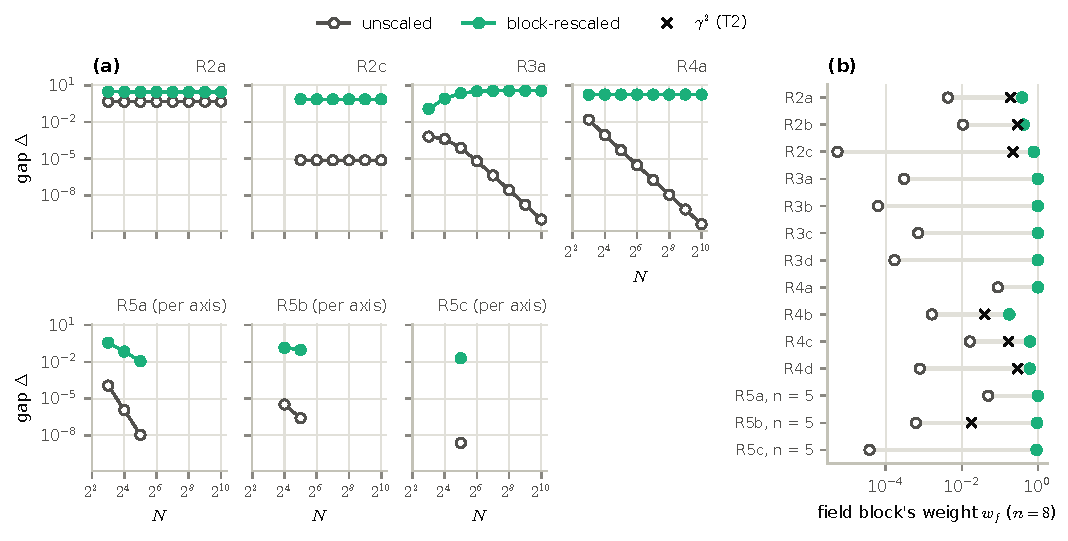
\includegraphics[width=\linewidth]{Figs/gap_rescaling.pdf}
    \caption[Block rescaling: the gap and the field block's weight]{\textbf{Block rescaling restores the descriptor's gap and the field block's weight on one axis; on two axes the gap still falls.} (a) The gap $\Delta$ on the physical subspace against $N$, unscaled (open) and block-rescaled (filled), for R2a and R2c (regular, R2c stiff), R3a and R4a (singular: the leading coefficient vanishes on $[-1,1]$) and R5a--R5c (two axes, per axis), at the resolutions whose reference is trusted. (b) For every panel at $n=8$ ($n=5$ per axis on R5), the field block's weight $w_f$ in the ground state, unscaled against rescaled, with the geometric initial state's overlap $\gamma^2\le w_f$ (crosses) where a preparation ran at that resolution: R2a--c, R4b--d and R5b; R3, R4a, R5a and R5c were prepared only at smaller $n$. Rescaling lifts the one-axis gaps to $\mathcal{O}(1)$ and $w_f$ towards one; on two axes it gains orders of magnitude but the gap still falls with $N$. Exact classical computations (the reference's spectrum); $\gamma^2$ from exact emulation (T2).}
    \label{fig:gap-rescaling}
\end{figure}

\paragraph{The stiff problem.} R2c, $f''+5f'+400f=0$, has the smallest unscaled gap and field weight of the regular problems, and rescaling gains most there. Rescaled, the descriptor prepares it from $n=5$, with infidelity $\res[2,sci]{stateprep/R2c/descriptor/n8/T2/filter=minimax}{infidelity}$ at $n=8$ by exact emulation. Its degree at $n=8$ is $\res[2,sci]{stateprep/R2c/descriptor/n8/T3/filter=minimax}{degree}$ against the standard form's $\res[2,sci]{stateprep/R2c/standard/n8/T3/filter=minimax}{degree}$ as built, and $\res[2,sci]{stateprep/R2c/descriptor/n8/T3/filter=minimax}{ideal_degree}$ against $\res[2,sci]{stateprep/R2c/standard/n8/T3/filter=minimax}{ideal_degree}$ at the ideal bound (T3). Unscaled, the gap and the field block's weight are each about five orders of magnitude smaller; how much more degree and amplification an unscaled preparation would need was not estimated, since rescaling also changes $\|\Hdesc\|$ and $\alpha_R$. The other problems, in both forms and at every tier, are given in \Cref{app:catalogue-results}.

Block rescaling therefore restores the gap the carried derivatives erode on every one-axis problem run, without ancilla; on two axes it only slows the gap's fall.

\subsection{Systems and Nonlinear Problems}
\label{sec:results-nonlinear}

\Cref{sec:extensions} claims that a Carleman lift is prepared where the doubled space only projects, and that the descriptor's lower degree survives on the lifted systems, where it enters through the time axis alone (\Cref{sec:prep-vs-proj}). The coupled oscillator R7 comes first, because every lift is a coupled linear system of its kind.

\paragraph{Two coupled fields.} The harmonic oscillator R7, $u'=v$, $v'=-\pi^2u$, is the realification of $z'=-\mathrm{i}\pi z$ (\Cref{sec:systems-complex}), carried as two fields on one state with its data as ratio rows. Both forms converge to rounding, the descriptor's field error $\res[2,sci]{build/R7/descriptor/n5}{field_err_linf}$ at $n=5$, and both prepare it: from $n=4$ the data-weighted geometric state has $\gamma^2=\res[3]{stateprep/R7/descriptor/n8/T2/filter=minimax}{gamma2}$ in the descriptor and $\res[3]{stateprep/R7/standard/n7/T2/filter=minimax}{gamma2}$ in the standard form, each at the largest $n$ it emulates, and every trusted exact emulation meets $\varepsilon$. The descriptor carries the system in its mass form, whose gap is about twice the block-rescaled chain's (\Cref{sec:systems-fields}) and which keeps the whole ground state on the field blocks, where the chain's derivative blocks take weight from them, $w_f=\res[3]{build/R7/descriptor/n8/layout=chain/chain}{field_weight}$. At $n=8$ the mass form's degree is $\res[2,sci]{stateprep/R7/descriptor/n8/T3/filter=minimax}{degree}$ against the standard form's $\res[2,sci]{stateprep/R7/standard/n8/T3/filter=minimax}{degree}$ as built and $\res[2,sci]{stateprep/R7/descriptor/n8/T3/filter=minimax}{ideal_degree}$ against $\res[2,sci]{stateprep/R7/standard/n8/T3/filter=minimax}{ideal_degree}$ at the ideal bound (T3), growing as $N$ against $N^2$ (\Cref{tab:catalogue-growth}). Simulated at $n=2$ on $\res{stateprep/R7/descriptor/n2/T1/filter=minimax}{n_qubits}$ qubits, where the reference is not yet trusted, the circuit agrees with the emulation to $\res[2,sci]{stateprep/R7/descriptor/n2/T1/filter=minimax}{filtered_agreement}$, a test of the circuit rather than of a preparation. What is prepared is the realified real system, at the cost of one field-register qubit; no complex residual was prepared (\Cref{sec:systems-complex}).

\paragraph{Projection against preparation.} The doubled space's kernel on R6a has dimension $\res{build/R6a/standard/n2}{kernel_count}$ at $n=2$ and $\res{build/R6a/standard/n5}{kernel_count}$ at $n=5$, in state spaces of $\res{build/R6a/standard/n2}{dimension}$ and $\res{build/R6a/standard/n5}{dimension}$ (\Cref{tab:doubled-kernel}), so a filter returns the initial state's projection onto it (\Cref{prop:no-penalty}), which is never a preparation. The Carleman lift of $y'=-y+y^2$ (R8) has a one-dimensional, trusted kernel at every order from $K=2$ to $6$ in both forms, so the filter prepares it.

\paragraph{The lift on a time axis (R8).} The field's error splits as \Cref{eq:carleman-error} predicts. At each order it is flat in $n_t$ from $n_t=3$, the time axis's part having fallen below the lift's, and it falls with the order, from $\res[2,sci]{build/R8/descriptor/n8/carleman=2}{field_err_linf}$ at $K=2$ to $\res[2,sci]{build/R8/descriptor/n8/carleman=6}{field_err_linf}$ at $K=6$, faster than the factor $\rho=\tfrac12$ per order that the bound of \Cref{sec:carleman} allows. Both forms prepare every order to $\varepsilon$; the infidelity at $K=4$ and $n_t=8$ is $\res[2,sci]{stateprep/R8/descriptor/n8/T2/carleman=4/filter=minimax}{infidelity}$ in the descriptor and $\res[2,sci]{stateprep/R8/standard/n8/T2/carleman=4/filter=minimax}{infidelity}$ in the standard form. The descriptor's time axis lowers the degree, by a margin that widens with $n_t$: at $K=4$ it is $\res{stateprep/R8/descriptor/n4/T2/carleman=4/filter=minimax}{degree}$ against $\res{stateprep/R8/standard/n4/T2/carleman=4/filter=minimax}{degree}$ at $n_t=4$ and $\res{stateprep/R8/descriptor/n8/T2/carleman=4/filter=minimax}{degree}$ against $\res{stateprep/R8/standard/n8/T2/carleman=4/filter=minimax}{degree}$ at $n_t=8$ by exact emulation, and $\res{stateprep/R8/descriptor/n4/T3/carleman=4/filter=minimax}{ideal_degree}$ against $\res{stateprep/R8/standard/n4/T3/carleman=4/filter=minimax}{ideal_degree}$ and $\res{stateprep/R8/descriptor/n8/T3/carleman=4/filter=minimax}{ideal_degree}$ against $\res{stateprep/R8/standard/n8/T3/carleman=4/filter=minimax}{ideal_degree}$ at the ideal bound (T3).

\paragraph{Burgers (R9): a trusted kernel can hide a diverging lift.} \Cref{fig:nonlinear-burgers} measures the lift's convergence on viscous Burgers from the data $a\sin x$, against the strength $a/\nu$ and the number of sine modes $M$, with $\nu=1$. The lift's error, its exact solution against the Galerkin system's, falls by a factor of about $a/(5\nu)$ per order: at $a/\nu=1$ from $\res[2,sci]{build/R9c-M4/descriptor/n5/carleman=2}{lift_err_linf}$ at $K=2$ to $\res[2,sci]{build/R9c-M4/descriptor/n5/carleman=5}{lift_err_linf}$ at $K=5$, and at $a/\nu=3$ from $\res[2]{build/R9d-M4/descriptor/n5/carleman=2}{lift_err_linf}$ to $\res[2]{build/R9d-M4/descriptor/n5/carleman=5}{lift_err_linf}$. It does not depend on $M$: at $a/\nu=1$ and $K=2$ it is $\res[2,sci]{build/R9c-M16/descriptor/n5/carleman=2}{lift_err_linf}$ on sixteen modes, as on four, while the worst-case ratio of \Cref{eq:carleman-ratio} grows from $\rho=\res[3]{panel/R9c-M4}{rho}$ to $\res[3]{panel/R9c-M16}{rho}$. The lift therefore converges at both ratios, though both exceed the bound's condition $\rho<1$, and its convergence follows $a/\nu$, not $\rho$. At $a/\nu=10$ it diverges, its error growing from $\res[3]{build/R9e-M4/descriptor/n5/carleman=2}{lift_err_linf}$ at $K=2$ to $\res[3]{build/R9e-M4/descriptor/n5/carleman=5}{lift_err_linf}$ at $K=5$ against an amplitude of $10$, while its kernel stays one-dimensional and trusted at every order, with gap ratio $\res[2,sci]{build/R9e-M4/descriptor/n5/carleman=5}{gap_ratio}$ at $K=5$. Both forms prepare it, with infidelity $\res[2,sci]{stateprep/R9e-M4/descriptor/n5/T2/carleman=5/filter=minimax}{infidelity}$ in the descriptor and $\res[2,sci]{stateprep/R9e-M4/standard/n5/T2/carleman=5/filter=minimax}{infidelity}$ in the standard form by exact emulation, and the decoded field is wrong by $\res[3]{stateprep/R9e-M4/descriptor/n5/T2/carleman=5/filter=minimax}{field_err_linf}$. This negative finding is analysed in \Cref{sec:carleman}: trust measures the kernel's isolation and says nothing of the lift's accuracy. The boundary lies between $a/\nu=3$ and $10$; that the factor $a/(5\nu)$ reaches one near $a/\nu=5$ is an extrapolation from these strengths, not a measurement. As on R8 the descriptor's time axis lowers the degree once $n_t$ grows: at $a/\nu=1$, $K=2$ and $n_t=5$ it is $\res{stateprep/R9c-M4/descriptor/n5/T2/carleman=2/filter=minimax}{degree}$ against the standard form's $\res{stateprep/R9c-M4/standard/n5/T2/carleman=2/filter=minimax}{degree}$ by exact emulation, and $\res{stateprep/R9c-M4/descriptor/n5/T3/carleman=2/filter=minimax}{ideal_degree}$ against $\res{stateprep/R9c-M4/standard/n5/T3/carleman=2/filter=minimax}{ideal_degree}$ at the ideal bound (T3). From $n_t=4$ it is the lower on every Burgers case estimated, $\res{time-axis/R9/n4}{lower}$ of $\res{time-axis/R9/n4}{pairs}$ at $n_t=4$ and $\res{time-axis/R9/n5}{lower}$ of $\res{time-axis/R9/n5}{pairs}$ at $n_t=5$; at $n_t=3$ it is the lower on only $\res{time-axis/R9/n3}{lower}$ of $\res{time-axis/R9/n3}{pairs}$ as built, the standard form winning at the stronger forcing and on more modes, as at $a/\nu=10$, $K=5$ on four modes, $\res{stateprep/R9e-M4/standard/n3/T3/carleman=5/filter=minimax}{degree}$ against $\res{stateprep/R9e-M4/descriptor/n3/T3/carleman=5/filter=minimax}{degree}$ (T3).

\begin{figure}[htbp]
    \centering
    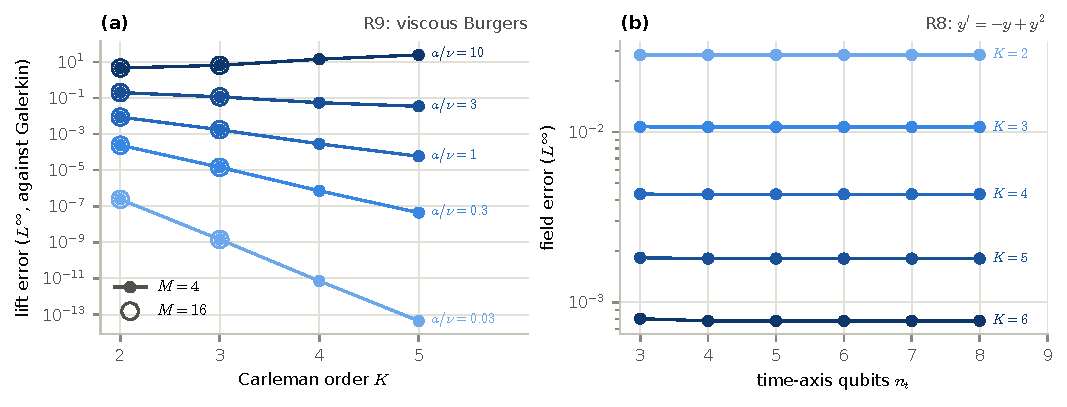
\includegraphics[width=\linewidth]{Figs/nonlinear_burgers.pdf}
    \caption[Convergence of the Carleman lift]{\textbf{The Carleman lift's convergence follows $a/\nu$, not $\rho$, and past it the kernel stays trusted while the lift diverges.} (a) Viscous Burgers (R9): the lift's error against the Galerkin system against the Carleman order $K$, at $a/\nu=0.03$, $0.3$, $1$, $3$ and $10$, to $K=5$ on $M=4$ sine modes (filled) and to $K=3$ on $M=16$ (rings). Where both are built the two coincide at plot scale, although $\rho$ grows with $M$, from $\res[3]{panel/R9c-M4}{rho}$ to $\res[3]{panel/R9c-M16}{rho}$ at $a/\nu=1$; at $a/\nu=10$ the error grows with $K$. (b) R8 ($y'=-y+y^2$, $\rho=\tfrac12$): the field's error against $n_t$ for $K=2$--$6$, flat at the lift's floor from $n_t=3$. Exact classical computations from the references; every trusted preparation of these lifts meets $\varepsilon$ by exact emulation (T2).}
    \label{fig:nonlinear-burgers}
\end{figure}

A Carleman lift is therefore prepared in both forms on every problem run, from R8 to Burgers, where the doubled space only projects. A preparation certifies the lift; whether the lift is the nonlinear solution is measured order by order, and on Burgers it fails at $a/\nu=10$ with no sign in the residual. From $n_t=4$ the descriptor's degree is the lower on every system and lift estimated, as built and at the ideal bound; on the coarsest time axes the standard form's can be the lower. \Cref{sec:results-ns} tests whether the advantage lasts as the coupling grows with the modes.

\subsection{Two-Dimensional Navier--Stokes}
\label{sec:results-ns}

\Cref{fig:navier-stokes} carries the lift to two-dimensional incompressible flow, the vorticity equation of \Cref{eq:navier-stokes} with $\nu=1$, prepared on $12$ to $48$ Fourier modes and built classically to $80$.

\paragraph{Validation.} The Taylor--Green vortex (R10a), whose two modes do not interact, has an exact lift, and the pipeline returns it to rounding: the lift's error is $\res[2,sci]{build/R10a-M12/descriptor/n4/carleman=2}{lift_err_linf}$ on twelve modes and $\res[2,sci]{build/R10a-M80/descriptor/n4/carleman=2}{lift_err_linf}$ on eighty. This checks the Galerkin coefficients, the ratio rows on the stated data and the time axis against a known answer; it does not test the lift's convergence, which the vortex pair does.

\paragraph{The vortex pair.} A counter-rotating pair of norm $\|w_0\|=a$ excites modes of several $|\mathbf k|$, so its triads are active. The truncation's own error against a direct simulation, about $\res[1,sci]{panel/R10b-M12}{truncation_err}$, $\res[1,sci]{panel/R10c-M12}{truncation_err}$ and $\res[1]{panel/R10d-M12}{truncation_err}$ on twelve modes at $a/\nu=3$, $10$ and $30$, is a property of the Galerkin system, not of the lift. The lift's error is set by the strength, as on Burgers (\Cref{fig:navier-stokes}); on twelve modes at $a/\nu=10$ it falls from $\res[2,sci]{build/R10c-M12/descriptor/n4/carleman=2}{lift_err_linf}$ at $K=2$ to $\res[2,sci]{build/R10c-M12/descriptor/n4/carleman=3}{lift_err_linf}$ at $K=3$. Unlike Burgers', it also grows with the modes: at $a/\nu=10$ and $K=2$ it is $\res[2]{build/R10c-M48/descriptor/n4/carleman=2}{lift_err_linf}$ on $48$ modes against $\res[2]{build/R10c-M12/descriptor/n4/carleman=2}{lift_err_linf}$ on twelve, though it still converges there, to $\res[2]{build/R10c-M48/descriptor/n4/carleman=3}{lift_err_linf}$ at $K=3$, at a $\rho$ of $\res[2]{panel/R10c-M48}{rho}$. At $a/\nu=30$ it converges on twelve modes, from $\res[3]{build/R10d-M12/descriptor/n4/carleman=2}{lift_err_linf}$ to $\res[3]{build/R10d-M12/descriptor/n4/carleman=3}{lift_err_linf}$, and diverges from $28$, where the error grows from $\res[3]{build/R10d-M28/descriptor/n4/carleman=2}{lift_err_linf}$ to $\res[3]{build/R10d-M28/descriptor/n4/carleman=3}{lift_err_linf}$ against $\|w_0\|=30$, as it does on $48$ (\Cref{fig:navier-stokes}), with every kernel trusted. This is the Burgers finding again, on a flow, and trust does not detect it. A shorter horizon, $T=\tfrac18$, restores convergence on $28$ modes, from $\res[3]{build/R10d-M28-W8/descriptor/n4/carleman=2}{lift_err_linf}$ to $\res[3]{build/R10d-M28-W8/descriptor/n4/carleman=3}{lift_err_linf}$, as the lift's time-dependent radius of convergence leads one to expect \cite{forets2017carleman}. Every trusted preparation by exact emulation meets $\varepsilon$, the worst at infidelity $\res[2,sci]{stateprep/R10d-M12-W8/descriptor/n4/T2/carleman=3/filter=minimax}{infidelity}$.

\paragraph{The time axis.} At one Carleman order the two forms differ only in the time axis (\Cref{sec:prep-vs-proj}), and the descriptor's degree is the lower in every pair estimated, $\res{time-axis/R10/n4}{pairs}$ at $n_t=4$ and $\res{time-axis/R10/n5}{pairs}$ at $n_t=5$, on $12$ to $48$ modes at $K=2$ to $4$ and $n_t=4$ and $5$, as built and at the ideal bound. A qubit of $n_t$ multiplies the standard form's degree by about four and the descriptor's by less than two: on the vortex pair at $a/\nu=10$, twelve modes and $K=2$, the degrees are $\res{stateprep/R10c-M12/standard/n4/T3/carleman=2/filter=minimax}{degree}$ and $\res{stateprep/R10c-M12/descriptor/n4/T3/carleman=2/filter=minimax}{degree}$ at $n_t=4$, and $\res{stateprep/R10c-M12/standard/n5/T3/carleman=2/filter=minimax}{degree}$ and $\res{stateprep/R10c-M12/descriptor/n5/T3/carleman=2/filter=minimax}{degree}$ at $n_t=5$. At fixed $n_t$ the margin narrows as the modes grow, because the coupling's part of the norm is common to both forms (\Cref{sec:prep-vs-proj}) and the descriptor's encoding of it loosens with its matchings: on $48$ modes the degrees are $\res{stateprep/R10c-M48/standard/n4/T3/carleman=2/filter=minimax}{degree}$ against $\res{stateprep/R10c-M48/descriptor/n4/T3/carleman=2/filter=minimax}{degree}$, and the descriptor's looseness $\alpha_R/\|R\|_2$ has grown from $\res[3]{looseness/stateprep/R10c-M12/descriptor/n4/T3/carleman=2/filter=minimax}{alpha_ratio}$ to $\res[3]{looseness/stateprep/R10c-M48/descriptor/n4/T3/carleman=2/filter=minimax}{alpha_ratio}$. The margin narrows at the ideal bound too, from $\res{stateprep/R10c-M12/standard/n4/T3/carleman=2/filter=minimax}{ideal_degree}$ against $\res{stateprep/R10c-M12/descriptor/n4/T3/carleman=2/filter=minimax}{ideal_degree}$ to $\res{stateprep/R10c-M48/standard/n4/T3/carleman=2/filter=minimax}{ideal_degree}$ against $\res{stateprep/R10c-M48/descriptor/n4/T3/carleman=2/filter=minimax}{ideal_degree}$, so part of the narrowing is the Hamiltonian's and part the encoder's.

\paragraph{The tier, and the tensor layout.} No circuit was simulated on Navier--Stokes. The narrowest prepared circuit, the descriptor at $n_t=4$ on twelve modes, has $\res{stateprep/R10a-M12/descriptor/n4/T3/carleman=2/filter=minimax}{n_qubits}$ qubits, wider than any circuit simulated here; the probe-verified reflections at $n_t=2$ are not prepared. The fluid results are therefore exact emulations, which equal the circuit's output (\Cref{sec:pipeline-verification}), and resource estimates. The tensor layout's coupling, the one native complex encoding built, keeps $2K-1$ terms whatever the number of modes and is verified by \gls{ir} to $\res{lift/R10c-M316/standard/n0/carleman=2/lift=tensor/verify=ir}{modes}$ modes, but prepares no state (\Cref{sec:systems-complex}); its gates per query against the matchings' are given in \Cref{tab:lift-circuits}.

\begin{figure}[htbp]
    \centering
    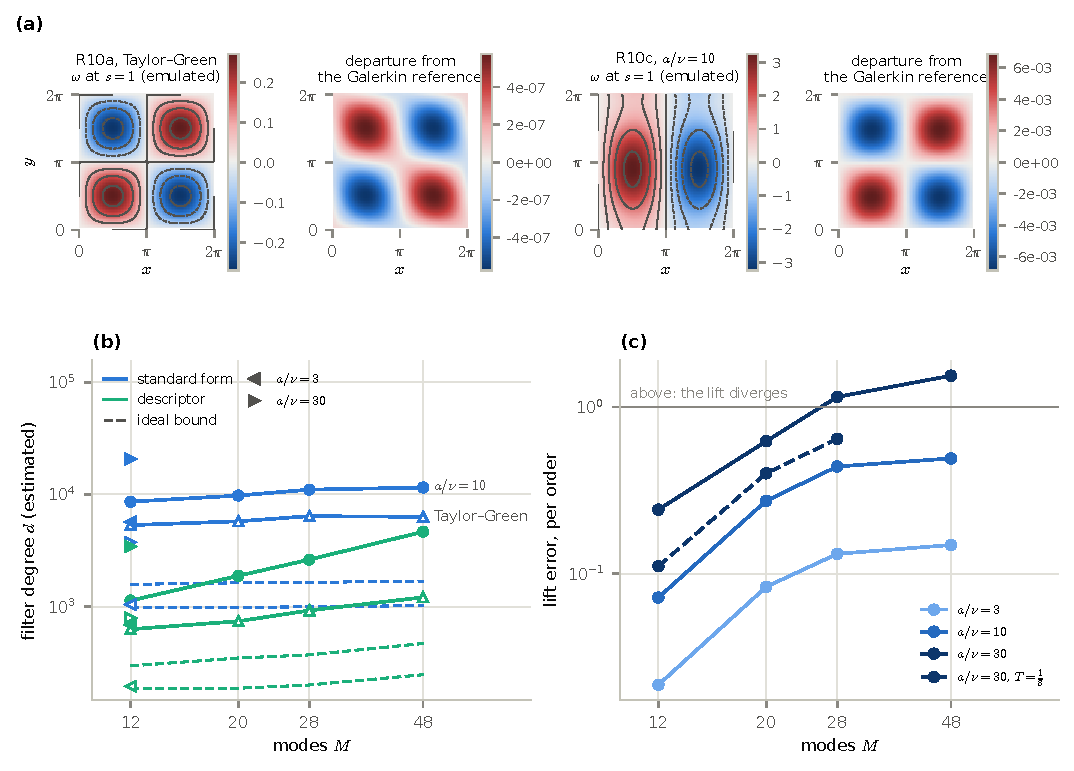
\includegraphics[width=\linewidth]{Figs/navier_stokes.pdf}
    \caption[Two-dimensional Navier--Stokes]{\textbf{Two-dimensional Navier--Stokes is prepared by exact emulation on up to 48 modes, and the descriptor's time axis lowers the degree in every pair.} (a) Vorticity at $t=T$: the field decoded from the prepared state against the Galerkin reference, for the Taylor--Green vortex (R10a, exact lift) and the vortex pair at $a/\nu=10$ (R10c), twelve modes, $K=3$, $n_t=4$; exact emulation (T2). (b) The minimax filter's degree against the number of modes $M$ at $K=2$, $n_t=4$, the form by colour, as built (solid) and at the ideal-encoding bound (dashed), over $M$ for the vortex pair at $a/\nu=10$ (circles) and the Taylor--Green vortex (open triangles), and on twelve modes, the only $M$ estimated at those strengths, for the pair at $a/\nu=3$ and $30$ (side-pointing triangles; filled as built, open at the ideal bound). The ratio of the two forms' degrees narrows as $M$ grows. (c) The lift's per-order error ratio against $M$ at $a/\nu=3$, $10$ and $30$ over $T=1$, and at $a/\nu=30$ over the window $T=\tfrac18$ on up to $28$ modes, with the line of unit ratio marked: above it the lift diverges while its kernel stays trusted. Resource estimates (T3) in (b); exact classical computations in (c). No circuit simulation (T1) was run on this problem.}
    \label{fig:navier-stokes}
\end{figure}

The lift therefore reaches two-dimensional incompressible flow by exact emulation on up to $48$ modes, with the descriptor's degree the lower in every pair, and with Burgers' caveat: at $a/\nu=30$ the lift diverges from $28$ modes with its kernel trusted.

\subsection{Summary of Findings}
\label{sec:results-summary}

\begin{enumerate}
    \item \textbf{The standard form's cost is its Hamiltonian's.} With Wu et al.'s encoding the degree on R2a grows as about $N^{10}$, mostly the encoder's cost; an exact encoding removes that part, and on one-axis problems with constant coefficients the degree still grows as $N^{2k}$, as built and at the ideal-encoding bound (\Cref{tab:headline,tab:growth}).
    \item \textbf{The descriptor's degree advantage depends on the class of problem.} Its degree grows as about $N$ on regular problems, as about $N^2$ on singular ones, and faster than $N^2$ per axis on two axes; per query it costs more gates than the structured encoding at small $n$ and about as many at $n=8$. \emph{Negative:} at the ideal bound the standard form needs the lower degree on R3, and on the heat equation at $n=4$ per axis, the two being level at $n=5$ (\Cref{sec:results-scaling}).
    \item \textbf{The descriptor's gap erodes where a carried derivative is uncontrolled, and block rescaling restores it on one axis only.} On every one-axis problem run the rescaled gap is $\mathcal{O}(1)$ and the field block regains its weight, without ancilla. \emph{Negative:} on two axes the rescaled gap still falls with $N$ (\Cref{sec:results-gap}).
    \item \textbf{The pipeline computes what it claims.} Every composed Hamiltonian of at most 24 qubits is verified whole and every lift and coupling by its terms; every circuit simulation with the minimax filter equals the exact emulation within $10^{-10}$; every trusted preparation meets $\varepsilon$, its a priori bound and its field budget. Wider reflections are built and counted but not independently verified (\Cref{sec:results-faithful}).
    \item \textbf{Coupled systems and Carleman lifts are prepared in both forms, but a trusted kernel can hide a diverging lift.} The mass form's gap is about twice the block-rescaled chain's on R7, and from $n_t=4$ the descriptor's degree is the lower on every system and lift estimated. \emph{Negative:} on Burgers at $a/\nu=10$, and on Navier--Stokes at $a/\nu=30$ from $28$ modes, the lift diverges while its kernel stays one-dimensional and trusted (\Cref{sec:results-nonlinear,sec:results-ns}).
    \item \textbf{Navier--Stokes is reached by exact emulation and resource estimate only.} Its narrowest prepared circuit is wider than any simulated, and the tensor layout's coupling, verified to \res{lift/R10c-M316/standard/n0/carleman=2/lift=tensor/verify=ir}{modes} modes, prepares nothing (\Cref{sec:results-ns}).
\end{enumerate}

Within its stated scope the central claim holds as measured: carrying the derivatives instead of eliminating them keeps the kernel and lowers the Hamiltonian's norm from $\Theta(N^8)$ to $\Theta(N^2)$ on a second-order equation with constant coefficients, and with it the degree from about $N^4$ to about $N$; the price is a block register and a gap the derivative blocks erode, which block rescaling restores on one axis without ancilla but not on two. \Cref{sec:discussion} gives the mechanism behind each finding and what the exponents imply beyond the benchmark problems.
